\chapter{Factor Attribution: PCA and Fama-French}
\label{ch:factors}

\begin{companioncode}{quant-factors}
Code: \texttt{crates/quant-factors/}\\
Dependencies: \crate{quant-core}, \crate{quant-timeseries}, \crate{quant-portfolio}, \crate{thiserror}\\
Run: \texttt{cargo run -p quant-factors --example pca\_demo}\\
Run: \texttt{cargo run -p quant-factors --example fama\_french}
\end{companioncode}

\section{Learning Objectives}

This chapter builds the factor attribution framework on top of the
covariance and CAPM machinery from \cref{ch:timeseries} and
\cref{ch:portfolio}: principal component analysis, the Fama-French
3-factor model, and risk decomposition. After completing it you can:

\begin{itemize}
    \item Explain why a single-factor model (CAPM) is insufficient and how
      multi-factor models capture additional systematic risk
    \item Compute the dominant eigenvalue and eigenvector of a symmetric
      matrix via the power method
    \item Deflate a matrix to find subsequent eigenpairs and recover the
      full spectrum
    \item Perform PCA on a returns matrix: centre, form the covariance,
      decompose, and project
    \item Quantify the explained variance ratio and the reconstruction
      error as a function of the number of retained components
    \item Estimate Fama-French 3-factor exposures (alpha, beta\_mkt,
      beta\_smb, beta\_hml) via OLS regression
    \item Decompose portfolio variance into systematic and idiosyncratic
      components
\end{itemize}

\begin{keyinsight}
CAPM says the market is the only systematic risk factor. Real returns
have multiple drivers: size (SMB), value (HML), momentum, quality. PCA
extracts the dominant statistical factors from the covariance matrix
without economic labels; the Fama-French model names three specific
factors with economic interpretation. The risk decomposition
$\sigma_p^2 = \text{systematic} + \text{idiosyncratic}$ tells you how
much of your portfolio's risk comes from factors you can hedge versus
asset-specific noise you must diversify away.
\end{keyinsight}

\section{Why Multi-Factor?}

\marginnote{%
\textbf{CAPM's blind spot}\\[0.3em]
CAPM says the market is the only systematic risk factor. Empirically,
small stocks and value stocks earn higher average returns than CAPM
predicts --- they carry systematic risk that the market beta does not
absorb. Multi-factor models name those additional risks so they can be
measured, hedged, and priced.
}

The CAPM of \cref{ch:portfolio} is a single-factor model: the expected
return of an asset is linear in its beta to the market portfolio alone.
Empirically, CAPM betas explain a modest fraction of the
cross-sectional variation in stock returns. Fama and French (1992)
showed that two additional factors --- \emph{size} (Small Minus Big,
SMB) and \emph{value} (High Minus Low, HML) --- capture systematic risk
that the market beta misses. Small stocks and value stocks earn higher
average returns than CAPM predicts, suggesting they carry additional
systematic risk that the market factor does not absorb.

\begin{marginfigure}
    \centering
    \vspace{-2cm}
    % Scree plot: explained variance per principal component.
% Usage: % Scree plot: explained variance per principal component.
% Usage: % Scree plot: explained variance per principal component.
% Usage: \input{figures/scree-plot}
% Scale: x = 1 cm per PC (3 PCs), y = 6 cm per unit EVR (0..1.0 -> 0..6 cm)
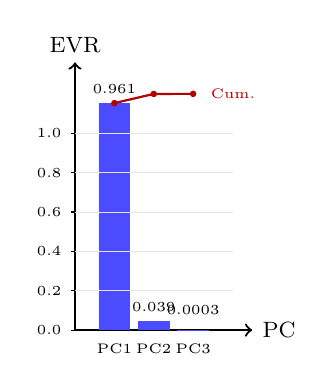
\begin{tikzpicture}[scale=0.5]
    % Axes
    \draw[thick, ->] (0,0) -- (4.5,0) node[right] {\footnotesize PC};
    \draw[thick, ->] (0,0) -- (0,6.8) node[above] {\footnotesize EVR};

    % Y-axis ticks
    \foreach \y/\ylab in {0/0.0, 1/0.2, 2/0.4, 3/0.6, 4/0.8, 5/1.0} {
        \draw (0,\y) -- (-0.1,\y);
        \node[left] at (-0.1,\y) {\tiny \ylab};
    }
    % X-axis labels
    \foreach \x/\xlab in {1/PC1, 2/PC2, 3/PC3} {
        \node[below] at (\x, -0.1) {\tiny \xlab};
    }

    % Bars: EVR = 0.9608, 0.0389, 0.0003 (scaled by 6)
    % PC1
    \fill[blue!70] (0.6, 0) rectangle (1.4, 5.765);
    \node[above] at (1.0, 5.765) {\tiny 0.961};
    % PC2
    \fill[blue!70] (1.6, 0) rectangle (2.4, 0.233);
    \node[above] at (2.0, 0.233) {\tiny 0.039};
    % PC3 (tiny, but still drawn)
    \fill[blue!70] (2.6, 0) rectangle (3.4, 0.002);
    \node[above] at (3.0, 0.15) {\tiny 0.0003};

    % Cumulative line (optional, shows the "knee")
    % Cumulative: 0.9608, 0.9997, 1.0000 (scaled by 6)
    \draw[thick, red!70!black, mark=*, mark size=1.5pt] plot coordinates {
        (1.0, 5.765) (2.0, 5.998) (3.0, 6.000)
    };
    \node[red!70!black, right] at (3.2, 6.0) {\tiny Cum.};

    % Grid lines (light)
    \foreach \y in {1,2,3,4,5} {
        \draw[gray!20, very thin] (0,\y) -- (4.0,\y);
    }
\end{tikzpicture}
% Scale: x = 1 cm per PC (3 PCs), y = 6 cm per unit EVR (0..1.0 -> 0..6 cm)
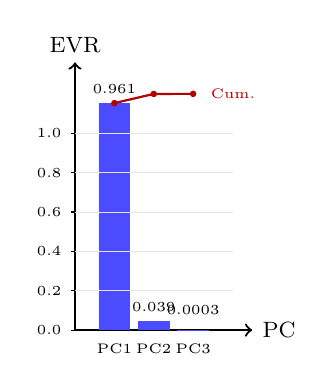
\begin{tikzpicture}[scale=0.5]
    % Axes
    \draw[thick, ->] (0,0) -- (4.5,0) node[right] {\footnotesize PC};
    \draw[thick, ->] (0,0) -- (0,6.8) node[above] {\footnotesize EVR};

    % Y-axis ticks
    \foreach \y/\ylab in {0/0.0, 1/0.2, 2/0.4, 3/0.6, 4/0.8, 5/1.0} {
        \draw (0,\y) -- (-0.1,\y);
        \node[left] at (-0.1,\y) {\tiny \ylab};
    }
    % X-axis labels
    \foreach \x/\xlab in {1/PC1, 2/PC2, 3/PC3} {
        \node[below] at (\x, -0.1) {\tiny \xlab};
    }

    % Bars: EVR = 0.9608, 0.0389, 0.0003 (scaled by 6)
    % PC1
    \fill[blue!70] (0.6, 0) rectangle (1.4, 5.765);
    \node[above] at (1.0, 5.765) {\tiny 0.961};
    % PC2
    \fill[blue!70] (1.6, 0) rectangle (2.4, 0.233);
    \node[above] at (2.0, 0.233) {\tiny 0.039};
    % PC3 (tiny, but still drawn)
    \fill[blue!70] (2.6, 0) rectangle (3.4, 0.002);
    \node[above] at (3.0, 0.15) {\tiny 0.0003};

    % Cumulative line (optional, shows the "knee")
    % Cumulative: 0.9608, 0.9997, 1.0000 (scaled by 6)
    \draw[thick, red!70!black, mark=*, mark size=1.5pt] plot coordinates {
        (1.0, 5.765) (2.0, 5.998) (3.0, 6.000)
    };
    \node[red!70!black, right] at (3.2, 6.0) {\tiny Cum.};

    % Grid lines (light)
    \foreach \y in {1,2,3,4,5} {
        \draw[gray!20, very thin] (0,\y) -- (4.0,\y);
    }
\end{tikzpicture}
% Scale: x = 1 cm per PC (3 PCs), y = 6 cm per unit EVR (0..1.0 -> 0..6 cm)
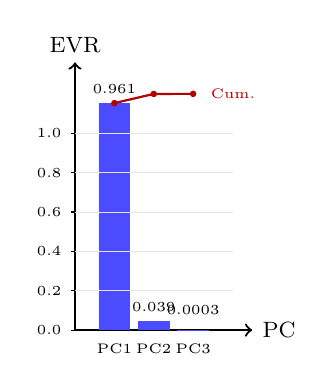
\begin{tikzpicture}[scale=0.5]
    % Axes
    \draw[thick, ->] (0,0) -- (4.5,0) node[right] {\footnotesize PC};
    \draw[thick, ->] (0,0) -- (0,6.8) node[above] {\footnotesize EVR};

    % Y-axis ticks
    \foreach \y/\ylab in {0/0.0, 1/0.2, 2/0.4, 3/0.6, 4/0.8, 5/1.0} {
        \draw (0,\y) -- (-0.1,\y);
        \node[left] at (-0.1,\y) {\tiny \ylab};
    }
    % X-axis labels
    \foreach \x/\xlab in {1/PC1, 2/PC2, 3/PC3} {
        \node[below] at (\x, -0.1) {\tiny \xlab};
    }

    % Bars: EVR = 0.9608, 0.0389, 0.0003 (scaled by 6)
    % PC1
    \fill[blue!70] (0.6, 0) rectangle (1.4, 5.765);
    \node[above] at (1.0, 5.765) {\tiny 0.961};
    % PC2
    \fill[blue!70] (1.6, 0) rectangle (2.4, 0.233);
    \node[above] at (2.0, 0.233) {\tiny 0.039};
    % PC3 (tiny, but still drawn)
    \fill[blue!70] (2.6, 0) rectangle (3.4, 0.002);
    \node[above] at (3.0, 0.15) {\tiny 0.0003};

    % Cumulative line (optional, shows the "knee")
    % Cumulative: 0.9608, 0.9997, 1.0000 (scaled by 6)
    \draw[thick, red!70!black, mark=*, mark size=1.5pt] plot coordinates {
        (1.0, 5.765) (2.0, 5.998) (3.0, 6.000)
    };
    \node[red!70!black, right] at (3.2, 6.0) {\tiny Cum.};

    % Grid lines (light)
    \foreach \y in {1,2,3,4,5} {
        \draw[gray!20, very thin] (0,\y) -- (4.0,\y);
    }
\end{tikzpicture}
    \caption{Scree plot: explained variance per principal component.
    The first PC captures 96\% of the total variance; the second adds
    3.9\%; the third adds only 0.3\%.}
    \label{fig:scree-plot}
\end{marginfigure}

A \emph{factor model} expresses each asset's excess return as a linear
combination of $K$ factor returns plus an idiosyncratic residual:
\[
  R_i - R_f = \alpha_i + \sum_{k=1}^{K} \beta_{ik} F_k + \varepsilon_i
\]
where $F_k$ is the return of factor $k$, $\beta_{ik}$ is the loading of
asset $i$ on factor $k$, and $\varepsilon_i$ is the asset-specific
residual. The factors are assumed to be uncorrelated with the
residuals, and the residuals are assumed uncorrelated across assets.

\section{Eigenvalue Decomposition: The Power Method}

The spectral theorem guarantees that every real symmetric matrix $A$
has an orthonormal basis of eigenvectors with real eigenvalues:
$A = V \Lambda V^\top$. The \emph{power method} finds the dominant
eigenpair $(\lambda_1, v_1)$ by repeated matrix-vector multiplication:
\[
  v^{(k+1)} = \frac{A v^{(k)}}{\|A v^{(k)}\|} \;\to\; v_1, \qquad
  \lambda_1 = v_1^\top A v_1 \quad \text{(Rayleigh quotient)}
\]
Starting from a random vector, each iteration amplifies the component
along $v_1$ by a factor $|\lambda_1 / \lambda_2|$ relative to the next
eigenvalue, so convergence is geometric with rate $|\lambda_2/\lambda_1|$.

\marginnote{%
\textbf{Power method intuition}\\[0.3em]
Repeated multiplication by $A$ amplifies the dominant eigendirection
the most. After $k$ steps, $v^{(k)} \propto \lambda_1^k v_1 +
\lambda_2^k v_2 + \ldots$ The ratio $|\lambda_2/\lambda_1|$ controls
convergence: well-separated spectra converge in a handful of
iterations; clustered eigenvalues are slow.
}

A sign-flip artefact arises when $\lambda_1 < 0$ (or when the initial
vector is exactly anti-aligned with the previous iterate): $v^{(k+1)}$
points opposite to $v^{(k)}$ while still converging in direction. We
fix this by aligning each iterate with its predecessor before testing
convergence, which makes the residual $\|v^{(k+1)} - v^{(k)}\|$
monotone non-increasing.

\begin{lstlisting}[language=Rust, caption={Power method for the dominant eigenpair.}]
pub fn power_method(
    matrix: &[Vec<f64>],
    max_iter: usize,
    tol: f64,
) -> Result<(f64, Vec<f64>), FactorError> {
    let n = matrix.len();
    let mut v = vec![1.0 / (n as f64).sqrt(); n];
    let mut lambda_prev = f64::INFINITY;
    for _ in 0..max_iter {
        let w = matvec_sym(matrix, &v);
        let norm = l2_norm(&w);
        let mut v_new: Vec<f64> = w.iter().map(|&x| x / norm).collect();
        // Align sign with the previous iterate to avoid spurious flips.
        let dot: f64 = v_new.iter().zip(v.iter()).map(|(a, b)| a * b).sum();
        if dot < 0.0 { for x in &mut v_new { *x = -*x; } }
        let av = matvec_sym(matrix, &v_new);
        let lambda: f64 = v_new.iter().zip(av.iter()).map(|(a, b)| a * b).sum();
        let delta = l2_norm(&v_new.iter().zip(v.iter())
            .map(|(a, b)| a - b).collect::<Vec<_>>());
        v = v_new;
        if (lambda - lambda_prev).abs() < tol && delta < tol * 10.0 {
            lambda_prev = lambda;
            break;
        }
        lambda_prev = lambda;
    }
    Ok((lambda_prev, v))
}
\end{lstlisting}

\section{Deflation and the Full Spectrum}

\marginnote{%
\textbf{Deflation trade-off}\\[0.3em]
Deflation is exact in infinite precision: $A' = A - \lambda v v^\top$
removes the eigendirection $v$ cleanly. In floating point, each
deflation step accumulates rounding error, so the smaller eigenvalues
are less accurate. For a well-conditioned $3 \times 3$ covariance,
the top two eigenpairs reach $10^{-6}$; the third may carry
$10^{-3}$ relative error. Use a QR/SVD solver if you need all
eigenpairs to full precision.
}

Once the dominant eigenpair is found, \emph{deflation} removes it from
the matrix:
\[
  A' = A - \lambda_1 \, v_1 v_1^\top
\]
For a symmetric matrix, $v_1 v_1^\top$ is the projector onto the
$e_1$ direction, so $A' v_1 = 0$ and the spectrum of $A'$ is
$\{0, \lambda_2, \lambda_3, \ldots\}$. Repeating the power method on
$A'$ yields $(\lambda_2, v_2)$, and so on.

\begin{lstlisting}[language=Rust, caption={Deflation and the top-$k$ eigenpairs.}]
pub fn deflate(
    matrix: &[Vec<f64>],
    eigenvalue: f64,
    eigenvector: &[f64],
) -> Vec<Vec<f64>> {
    let n = matrix.len();
    let mut out = vec![vec![0.0; n]; n];
    for i in 0..n {
        for j in 0..n {
            out[i][j] = matrix[i][j] - eigenvalue * eigenvector[i] * eigenvector[j];
        }
    }
    out
}

pub fn top_k_eigen(matrix: &[Vec<f64>], k: usize)
    -> Result<(Vec<f64>, Vec<Vec<f64>>), FactorError>
{
    let mut current = matrix.to_vec();
    let mut eigenvalues = Vec::with_capacity(k);
    let mut eigenvectors = Vec::with_capacity(k);
    for _ in 0..k {
        let (lambda, v) = power_method(&current, 0, 0.0)?;
        eigenvalues.push(lambda);
        eigenvectors.push(v.clone());
        current = deflate(&current, lambda, &v);
    }
    Ok((eigenvalues, eigenvectors))
}
\end{lstlisting}

The accumulated floating-point error in deflation limits the accuracy
of the smaller eigenvalues. For a well-conditioned matrix with
well-separated eigenvalues, the top two or three eigenpairs are
accurate to $10^{-6}$; the last eigenpair of a near-singular matrix
may carry relative error of $10^{-3}$ or worse.

\section{PCA: Covariance Eigendecomposition}

\marginnote{%
\textbf{Why centre?}\\[0.3em]
Subtracting the per-column mean before forming $\Sigma$ removes the
``level'' component. Without centring, the first PC would just pick up
the mean return direction; with centring, the first PC captures the
direction of maximum \emph{variance} around that mean --- which is
what we want for risk analysis.
}

\marginnote{%
\textbf{EVR denominator}\\[0.3em]
Use $\text{tr}(\Sigma) = \sum_{j=1}^{N} \lambda_j$, the \emph{full}
covariance trace --- not $\sum_{j=1}^{k} \lambda_j$ over retained
components only. With the full trace, $\sum_i \text{EVR}_i < 1$ when
$k < N$, which is the correct statement: retained components explain
\emph{this fraction} of total variance.
}

Given a returns matrix $X$ ($T$ observations $\times$ $N$ assets), PCA
centres the data by subtracting the per-column mean, forms the sample
covariance $\Sigma = \frac{1}{T-1} \tilde{X}^\top \tilde{X}$, and
decomposes it as $\Sigma = V \Lambda V^\top$. The principal components
are the columns of $V$ (the eigenvectors), and the explained variance
ratio of component $i$ is
\[
  \text{EVR}_i = \frac{\lambda_i}{\text{tr}(\Sigma)}
  = \frac{\lambda_i}{\sum_{j=1}^{N} \lambda_j}
\]
where $\text{tr}(\Sigma) = \sum_j \lambda_j$ is the total variance.
The cumulative explained variance after $k$ components is
$\sum_{i=1}^{k} \text{EVR}_i$.

\begin{lstlisting}[language=Rust, caption={PCA fit: centre, covariance, eigendecompose.}]
pub fn pca(returns: &[Vec<f64>], n_components: usize)
    -> Result<PcaResult, FactorError>
{
    let (t, n) = (returns.len(), returns[0].len());
    let mean: Vec<f64> = (0..n)
        .map(|j| returns.iter().map(|r| r[j]).sum::<f64>() / t as f64)
        .collect();
    let mut cov = vec![vec![0.0; n]; n];
    for row in returns {
        for i in 0..n {
            let di = row[i] - mean[i];
            for j in 0..n { cov[i][j] += di * (row[j] - mean[j]); }
        }
    }
    let denom = (t - 1) as f64;
    for row in &mut cov { for cell in row.iter_mut() { *cell /= denom; } }
    let (eigenvalues, eigenvectors) = top_k_eigen(&cov, n_components)?;
    let trace: f64 = (0..n).map(|i| cov[i][i]).sum();
    let explained_variance_ratio: Vec<f64> =
        eigenvalues.iter().map(|&l| l / trace).collect();
    Ok(PcaResult { eigenvalues, eigenvectors, explained_variance_ratio,
        cumulative_variance: /* ... */, mean })
}
\end{lstlisting}

\begin{lstlisting}[language=Rust, caption={Project and reconstruct.}]
pub fn pca_transform(returns: &[Vec<f64>], eigenvectors: &[Vec<f64>],
                    mean: &[f64]) -> Vec<Vec<f64>> {
    returns.iter().map(|row| {
        let centred: Vec<f64> = row.iter().zip(mean.iter())
            .map(|(x, m)| x - m).collect();
        eigenvectors.iter().map(|pc|
            pc.iter().zip(centred.iter()).map(|(a, b)| a * b).sum()
        ).collect()
    }).collect()
}

pub fn pca_reconstruct(scores: &[Vec<f64>], eigenvectors: &[Vec<f64>],
                       mean: &[f64]) -> Vec<Vec<f64>> {
    scores.iter().map(|row| {
        let mut out = mean.to_vec();
        for (k, score) in row.iter().enumerate() {
            for (out_j, ev) in out.iter_mut().zip(eigenvectors[k].iter()) {
                *out_j += score * ev;
            }
        }
        out
    }).collect()
}
\end{lstlisting}

\subsection{Demo Results}

Running \texttt{pca\_demo} on 12 synthetic observations of 3 assets
yields the following decomposition:

\begin{center}
\begin{tabular}{lrrr}
\toprule
PC & Eigenvalue & EVR & Cumulative \\
\midrule
1 & $1.96 \times 10^{-4}$ & 0.9608 & 0.9608 \\
2 & $7.94 \times 10^{-6}$ & 0.0389 & 0.9997 \\
3 & $7.00 \times 10^{-8}$ & 0.0003 & 1.0000 \\
\bottomrule
\end{tabular}
\end{center}

The top eigenvector $v_1 \approx (0.892, 0.452, -0.022)$ shows that the
first PC is essentially a long-asset-1, long-asset-2 position ---
the dominant source of co-movement. The reconstruction error (SSE)
decreases from $8.8 \times 10^{-5}$ (1 component) to $7.2 \times 10^{-7}$
(2 components) to $\approx 0$ (3 components), confirming the
$1/\sqrt{k}$ intuition.

\section{Fama-French 3-Factor Regression}

The Fama-French model regresses asset excess returns on three factors:
\[
  R_i - R_f = \alpha_i + \beta_{\text{Mkt}} (R_m - R_f)
  + \beta_{\text{SMB}} \cdot \text{SMB}
  + \beta_{\text{HML}} \cdot \text{HML}
  + \varepsilon_i
\]
The design matrix is $X = [1, \text{Mkt-Rf}, \text{SMB}, \text{HML}]$
and the OLS fit reuses the Gaussian-elimination solver from
\crate{quant-timeseries}.

\marginnote{%
\textbf{Alpha = skill or noise?}\\[0.3em]
The intercept $\alpha_i$ is the average return left over after the
three factors explain what they can. In-sample, any asset has a
non-zero alpha by construction; the question is whether it is
statistically different from zero out-of-sample. In a well-specified
factor model, alphas should be small and mostly insignificant.
}

\marginnote{%
\textbf{Partial vs simple regression}\\[0.3em]
$\beta_{\text{Mkt}}$ from FF3 is a \emph{partial} coefficient: it
measures market exposure \emph{after} controlling for SMB and HML. It
differs from the CAPM beta (a simple regression on the market alone)
whenever the factors are correlated. Do not expect FF3 $\beta_{\text{Mkt}}$
to equal CAPM $\beta$.
}

\begin{lstlisting}[language=Rust, caption={FF3 regression via the OLS machinery.}]
pub fn ff3_regression(asset_excess: &[f64], factors: &[Vec<f64>])
    -> Result<FF3Exposure, FactorError>
{
    let x: Vec<Vec<f64>> = factors.iter()
        .map(|row| vec![1.0, row[0], row[1], row[2]])
        .collect();
    let fit = ols(&x, asset_excess)
        .map_err(|e| FactorError::Singular(e.to_string()))?;
    let n = asset_excess.len() as f64;
    let dof = (n - 4.0).max(1.0);
    let residual_var = fit.residuals.iter()
        .map(|e| e * e).sum::<f64>() / dof;
    Ok(FF3Exposure {
        alpha: fit.coeffs[0],
        beta_mkt: fit.coeffs[1],
        beta_smb: fit.coeffs[2],
        beta_hml: fit.coeffs[3],
        r_squared: fit.r_squared,
        residual_var,
    })
}
\end{lstlisting}

\subsection{Demo Results}

Running \texttt{fama\_french} on 100 simulated observations with the
DGP $\alpha = 0.001$, $\beta_{\text{Mkt}} = 1.2$,
$\beta_{\text{SMB}} = 0.4$, $\beta_{\text{HML}} = -0.3$ plus noise:

\begin{center}
\begin{tabular}{lrr}
\toprule
Parameter & True & Estimated \\
\midrule
$\alpha$ & 0.001 & 0.001003 \\
$\beta_{\text{Mkt}}$ & 1.2 & 1.2008 \\
$\beta_{\text{SMB}}$ & 0.4 & 0.4016 \\
$\beta_{\text{HML}}$ & $-0.3$ & $-0.2977$ \\
$R^2$ (FF3) & --- & 0.9893 \\
$R^2$ (CAPM) & --- & 0.9391 \\
\bottomrule
\end{tabular}
\end{center}

The 3-factor model's $R^2$ (98.9\%) beats the single-factor CAPM's
$R^2$ (93.9\%) by 5.3 percentage points --- the incremental explanatory
power of SMB and HML beyond the market.

\section{Risk Attribution}

\marginnote{%
\textbf{Systematic vs idiosyncratic}\\[0.3em]
Systematic risk comes from factors you can hedge (market, size, value)
--- it is shared across assets and does not diversify away.
Idiosyncratic risk is asset-specific noise; it does diversify away as
$N$ grows. A well-diversified portfolio has $\sigma_p^2$ dominated by
the systematic term.
}

Given portfolio weights $w$, factor loadings $B$ ($N \times K$), factor
covariance $\Sigma_F$ ($K \times K$), and per-asset idiosyncratic
variances $D$ (diagonal), the portfolio variance decomposes as
\[
  \sigma_p^2 = \underbrace{w^\top B \, \Sigma_F \, B^\top w}_{\text{systematic}}
  + \underbrace{w^\top D \, w}_{\text{idiosyncratic}}
\]
The portfolio's factor exposure is $f_p = B^\top w$ (a $K$-vector);
the systematic variance is $f_p^\top \Sigma_F f_p$; the per-factor
contribution is the diagonal approximation
$\text{contrib}_k = f_{p,k}^2 \, \Sigma_{F,kk}$.

\begin{lstlisting}[language=Rust, caption={Risk attribution.}]
pub fn risk_attribution(
    weights: &[f64],
    factor_loadings: &[Vec<f64>],
    factor_covariance: &[Vec<f64>],
    residual_variances: &[f64],
) -> Result<RiskAttribution, FactorError> {
    let n = weights.len();
    let k = factor_loadings[0].len();
    // Portfolio factor exposures: f_p[k] = sum_i w_i * beta_ik.
    let mut f_p = vec![0.0; k];
    for (i, w_i) in weights.iter().enumerate() {
        for (kk, &beta) in factor_loadings[i].iter().enumerate() {
            f_p[kk] += w_i * beta;
        }
    }
    // Systematic: f_p' Sigma_F f_p.
    let mut systematic = 0.0;
    for i in 0..k {
        for j in 0..k {
            systematic += f_p[i] * factor_covariance[i][j] * f_p[j];
        }
    }
    // Idiosyncratic: sum_i w_i^2 * D_i.
    let idiosyncratic: f64 = weights.iter()
        .zip(residual_variances.iter())
        .map(|(w, d)| w * w * d).sum();
    let factor_contributions: Vec<f64> = (0..k)
        .map(|kk| f_p[kk] * f_p[kk] * factor_covariance[kk][kk])
        .collect();
    Ok(RiskAttribution {
        total_variance: systematic + idiosyncratic,
        systematic_variance: systematic,
        idiosyncratic_variance: idiosyncratic,
        factor_contributions,
    })
}
\end{lstlisting}

For the FF3 demo, the risk attribution on the single-asset portfolio
($w = 1$) gives:

\begin{center}
\begin{tabular}{lr}
\toprule
Component & Variance \\
\midrule
Total & $8.94 \times 10^{-5}$ \\
Systematic & $8.84 \times 10^{-5}$ (98.9\%) \\
Idiosyncratic & $9.85 \times 10^{-7}$ (1.1\%) \\
\midrule
Mkt contribution & $8.41 \times 10^{-5}$ \\
SMB contribution & $3.40 \times 10^{-6}$ \\
HML contribution & $8.54 \times 10^{-7}$ \\
\bottomrule
\end{tabular}
\end{center}

The market factor dominates the systematic variance (95.1\% of
total), consistent with the large market beta ($\beta_{\text{Mkt}} = 1.2$)
and the large market variance.

\section{Exercises}

\begin{enumerate}
    \item Add a 4th and 5th factor (momentum, quality) to the FF
      regression and compare $R^2$ to the 3-factor model.
    \item Implement the Jacobi eigenvalue algorithm as an alternative
      to the power method and compare convergence on a $5 \times 5$
      covariance matrix.
    \item Run PCA on a real equity returns matrix (e.g., 10 stocks,
      252 days) and interpret the first three principal components
      economically.
    \item Compute the rolling 60-day beta of a stock to the market
      factor and plot the time series.
    \item Construct a long-short portfolio that is neutral to the
      market ($\beta_{\text{Mkt}} = 0$) but exposed to SMB, and
      decompose its risk into systematic and idiosyncratic parts.
\end{enumerate}

\section{Key Takeaways}

\begin{itemize}
    \item The power method finds the dominant eigenpair in
      $O(n^2)$ per iteration; deflation extends it to the full spectrum
      at the cost of accumulated floating-point error.
    \item PCA centres the data, decomposes the covariance, and ranks
      components by explained variance; the reconstruction error
      decreases as more components are retained.
    \item The Fama-French 3-factor model adds size (SMB) and value
      (HML) to the market factor; the $R^2$ improvement over CAPM
      quantifies the incremental explanatory power.
    \item Risk decomposition splits portfolio variance into
      systematic (factor-driven) and idiosyncratic (asset-specific)
      parts; diversification eliminates the idiosyncratic part.
    \item The power method's sign-flip artefact is handled by aligning
      each iterate with its predecessor before testing convergence.
\end{itemize}